\documentclass[12pt]{article}
\usepackage{setspace}  % To use linespacing
\usepackage{indentfirst} % Indents first line after sections
\usepackage{amssymb} % For \mathbb
\usepackage{enumerate} % For changing labels of enumerate
\usepackage[margin=1in]{geometry} % For editing margins
\usepackage{tikz} % Tikz drawing for graphs
\usetikzlibrary{arrows.meta} % Allows customizing arrows
\usetikzlibrary{backgrounds} % For framing a tikzpicture
\usetikzlibrary{calc, through}
\usetikzlibrary{decorations.markings}
\usetikzlibrary{arrows}
\usetikzlibrary{positioning}
\usepackage{amsmath}
\usepackage{ifthen}
\usepackage{intcalc} % \intcalcMod

% Make new commands
\newcommand{\N}{\mathbb{N}}
\newcommand{\R}{\mathbb{R}}
\newcommand{\Z}{\mathbb{Z}}
\newcommand{\abs}[1]{\left|#1\right|}
\newcommand{\paren}[1]{\left(#1\right)}
\newcommand{\fivespace}{\space\space\space\space\space}

\newcommand{\be}{\begin{enumerate}}
\newcommand{\ee}{\end{enumerate}}
\newcommand{\seti}[1]{\setcounter{enumi}{#1}}
\newcommand{\setii}[1]{\setcounter{enumii}{#1}}

% Start main document
\begin{document}
\onehalfspacing
\hfill Frank Cline

\hfill Math 307

\hfill HW 9

% PROBLEMS
\section*{Problems 1-4}

\be
% 1
\item Find a plane drawing of the following graphs. Label your graph to demonstrate the isomorphism. For the left-hand graph, can you find a plane embedding with mirror symmetry?

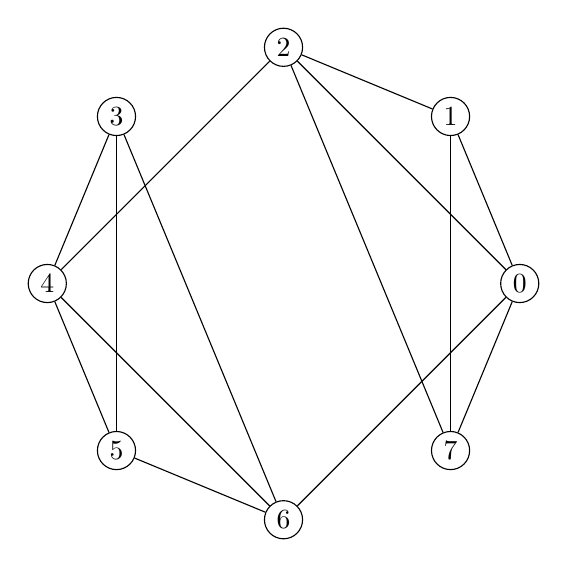
\begin{tikzpicture}
\foreach \i in {0, 1, ..., 7}{\node[draw, circle, inner sep = 2pt] (\i) at (360*\i/8: 3){\i};}
\foreach  \i/\j in {0/1, 0/2, 0/6, 0/7, 1/2, 1/7, 2/4, 2/7, 3/4, 3/5, 3/6, 4/5, 4/6, 5/6}
{\draw (\i) -- (\j);}
\end{tikzpicture}
\hspace{2cm}
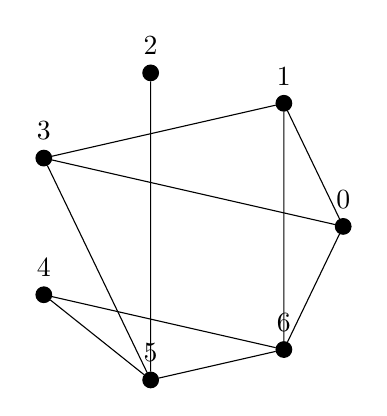
\begin{tikzpicture}[]
\foreach \i in {0, ...,6}{  \node[draw, circle, fill=black, inner sep = 2 pt, label={$\i$}](\i) at (\i*360/7: 2) {};}
\draw (1) -- (3)--(0);
\draw (2) -- (5) -- (4) -- (6) -- (0) --(1)--(6);
\draw (3) -- (5)--(6);
 \end{tikzpicture}

	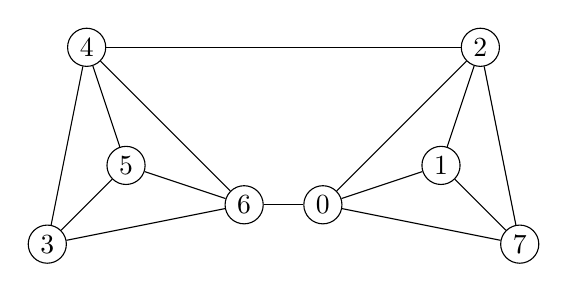
\begin{tikzpicture}
	\begin{scope}[every node/.style={circle, draw, inner sep = 2pt}]
	    	\node (2) at (3,0) {2};
		\node (1) at (2.5,-1.5) {1};
	    	\node (0) at (1,-2) {0};
		\node (7) at (3.5,-2.5) {7};
		\node (4) at (-2,0) {4};	
		\node (6) at (0,-2) {6};
		\node (3) at (-2.5,-2.5) {3};
		\node (5) at (-1.5,-1.5) {5};
	\end{scope}
	
	\begin{scope}[>={Stealth[black]},
	              every node/.style={fill=white,circle},
	              every edge/.style={draw=black}]
		\path (0) edge (1);
		\path (0) edge (2);
		\path (0) edge (6);
		\path (0) edge (7);
		\path (1) edge (7);
		\path (2) edge (1);
		\path (2) edge (4);
		\path (2) edge (7);
		\path (3) edge (4);
		\path (3) edge (5);
		\path (3) edge (6);
		\path (4) edge (5);
		\path (4) edge (6);
		\path (5) edge (6);
	\end{scope}
	\end{tikzpicture}
	\hspace{2cm}
		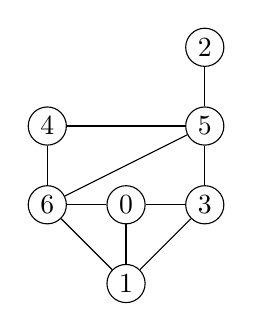
\begin{tikzpicture}
	\begin{scope}[every node/.style={circle, draw, inner sep = 2pt}]
	    	\node (0) at (0,1) {0};
		\node (1) at (0,0) {1};
	    	\node (2) at (1,3) {2};
	    	\node (3) at (1,1) {3};
	    	\node (4) at (-1,2) {4};
	    	\node (5) at (1,2) {5};
	    	\node (6) at (-1,1) {6};
	\end{scope}
	
	\begin{scope}[>={Stealth[black]},
	              every node/.style={fill=white,circle},
	              every edge/.style={draw=black}]
		\path (0) edge (1);
		\path (0) edge (3);
		\path (0) edge (6);
		\path (1) edge (3);
		\path (1) edge (6);
		\path (2) edge (5);
		\path (3) edge (5);
		\path (4) edge (5);
		\path (4) edge (6);
		\path (5) edge (6);
	\end{scope}
	\end{tikzpicture}
\ee

\end{document}















